\section{The HARP framework}

In this Section, firstly, a brief overview of the HARP framework for graph coarsening \cite{chen_harp_2018} is presented, followed by our analysis of the properties of graph coarsenings in general.

\subsection{HARP}
\todo[inline]{Explanation of the general structure of HARP, without going into detail about the coarsening procedure}
HARP is a method for improving the performance of graph representation learning (i.e. graph embedding) algorithms such as DeepWalk \cite{perozzi_deepwalk_2014}, LINE \cite{tang_line_2015}, PTE \cite{tang_pte_2015} or node2vec \cite{grover_node2vec_2016}. The method is a combination of dataset augmentation and pre-training based on the general principle that graph-based models train more efficiently on smaller graphs and can thus be pre-trained on a coarsened representation of the graph at hand. Moreover, the coarsened graphs approximate the global properties of the original data, enabling the representations to better encapsulate such a global structure. In an overview, the method consists of the following steps:

Consider an undirected graph \( G \) with nodes \( V \left( G \right) \) and edges \( E \left( G \right) \). The aim of the graph coarsening part of the algorithm is to generate a sequence of graphs \( G_0, G_1, G_2, \dots, G_L \) where \( G_0 = G \) and \( L \in \mathfield{N} \) is a hyper-parameter of the method. In this sequence, each graph \( G_i \) is generated from the graph \( G_{i - 1} \) by coarsening it -- lowering the number of nodes and edges while preserving the general structure of the graph. Following \cite{chen_harp_2018}, let \( \psi_i \) denote the mapping between the graphs such that \( V \left( G_i \right) = \psi_i \left( V \left( G_{i - 1} \right) \right) \).

\begin{itemize}
  \item \textbf{Dataset augmentation}. The graph \( G \) is consecutively reduced in size by the application of several graph coarsening schemas. In each step, the coarsened graph can be viewed as an ever coarser representation of the graph data and its global structure. This step can be run ahead-of-time to produce the resulting coarsened graphs \( G_0, G_1, \dots, G_L \).
\end{itemize}
After all the coarsened graphs are pre-computed, the method itself can be executed by repeating the following steps on the graphs from the coarsest to the finest (i.e. from \( G_L \) to \( G_0 \)):
\begin{itemize}
  \item \textbf{Training on an intermediary graph}. The graph embedding model is trained on \( G_i \), producing \( \Phi_{G_i} \), an embedding of the graph in a Euclidean space.
  \item \textbf{Embedding prolongation}. The embedding \( \Phi_{G_i} \) is prolonged from the current graph to one that is one step closer to \( G_0 \), yielding \( \Phi_{G_{i - 1}} \). This embedding is used as the starting state for the graph model which is to be trained on \( G_{i - 1} \).
\end{itemize}
These steps are repeated until \( \Phi_{G_0} \) is computed. While the training step of this schema is a straightforward application of one of the aforementioned embedding algorithms to \( G_i \), the particular details of the coarsening and prolongation steps are further explained in Sections \ref{sec:adaptive-prolongation} and \ref{sec:harp-coarsening}.

The first step is independent of the rest of the computation and can be done ahead of time. The last two steps can be seen as a form of pre-training for the model that is to be learnt on the original graph. The whole HARP pipeline is demonstrated in Figure \ref{fig:harp-overview}.\todo{The image isn't exactly correct}

\begin{figure}
  \centering
  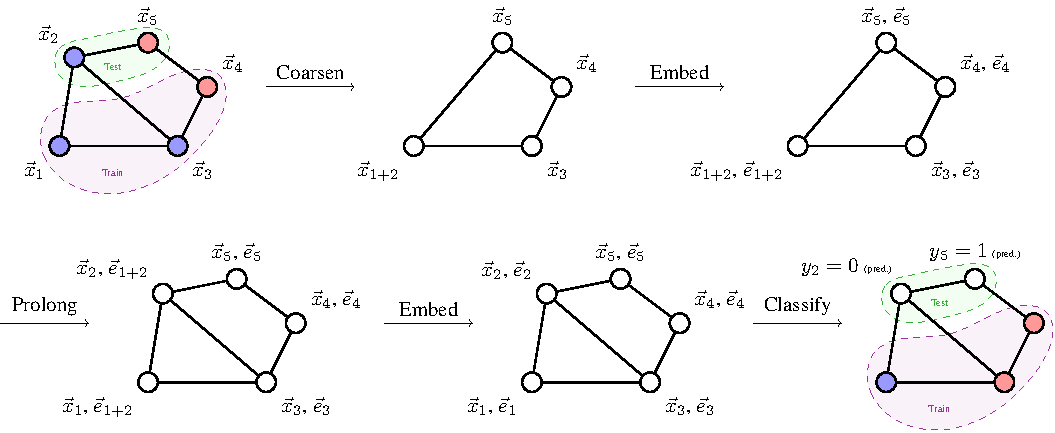
\includegraphics[width=\linewidth]{images/harp-overview/harp-overview.pdf}
  \caption{An overview of the HARP processing pipeline with one level of coarsening}
  \label{fig:harp-overview}
\end{figure}
